\chapter{Results of Workflow Validation}\label{chap:results}
The Galaxy workflows are validated using real-world datasets from different laboratories. The analysis results for each workflow with complying test samples are described below.

\section{Poxvirus Workflow with Lumpy Skin Disease Virus Datasets}
We employed our pipeline using a tiling amplicon approach with masked reference sequences for each half genome to ensure an unambiguous mapping to the two \ac{ITR} regions of the poxvirus genome. Two public \ac{LSDV} samples, 20L70 (MZ577075.1) and 20L81 (MZ577076.1), that were sequenced with the required tiled amplicon method in two pools are used and retrieved from GenBank on 10\textsuperscript{th} April, 2023. Collected from cattle in 2020 during a lumpy skin disease outbreak in Northern Vietnam (20L70\_Dinh-To/VNM/20 and 20L81\_Bang-Thanh/VNM/20), both samples were sequenced on a MiSeq System using a Nextera XT library preparation kit. Recent research revealed the presence of non-Neethling strains in samples from recombinant vaccine-like \ac{LSDV} genomes, and the two samples are shown to be from this recombinant strain~\cite{vandenbussche2022recombinant}. This indicates that the hosts were vaccinated with the concerned vaccine Lumpivax, what suggests that the resulting recombinant genome can be reliably mapped to other viruses belonging to the Capripoxvirus family. \\
The used \acs{CaPV} primer scheme in \ac{BED} format contains information about the primer pairs used for the amplicons. Each primer pair has one positive and one negative strand primer, indicated by the strand in the sixth column and by the \textit{LEFT} and \textit{RIGHT} label in the name. Primers are labeled in an alternating way, \textit{pool1} primer pairs are denoted as \textit{pool1a} and \textit{pool1b}. We use the same method for \textit{pool2} with \textit{pool2a} and \textit{pool2b}. We reuse the \textit{SCORE} column from the \ac{BED} file to unambiguously identify primer and strand for each amplicon. The annotated primer scheme for \ac{CaPV} is part of the workflow run to which links are provided in Supplementary~\secref{sec:apx-aiv-links}. The \ac{LSDV} ``Neethling'' strain was used as reference genome (NC\_003027.1) for mapping. The raw FASTQ files for each sample were quality trimmed with \texttt{fastp} and mapped to each half-masked reference, which is explained in detail below.
\\

\setlength{\tabcolsep}{16pt}
\renewcommand{\arraystretch}{1.3}
\begin{table}[ht!]
    \centering
    \begin{tabular}{lcc}
    \toprule
    \textbf{Output Metric}                      & \textbf{20L70}     & \textbf{20L81}     \\ \midrule
    Paired-end raw reads                        & 863 820            & 1 016 168          \\ 
    Paired-end reads after quality trimming     & 856 138            & 947 064            \\ \midrule
    Proportion of reads mapping to reference    & 99.6\%             & 77.3\%             \\ 
    Proportion of reference covered             & 99.68\%            & 99.68\%            \\ \midrule
    Mean coverage                               & 2 705.2 \texttimes & 2 411.4 \texttimes \\ 
    Alignment error rate                        & 1.25\%             & 1.30\%             \\ \bottomrule
    \end{tabular}
    \caption{Metrics after preprocessing and mapping for datasets 20L70 and 20L81.}
    \label{tab:4-pox-metrics}
\end{table}

\begin{figure}[ht!]
    \centering
    \hspace*{-8pt}
    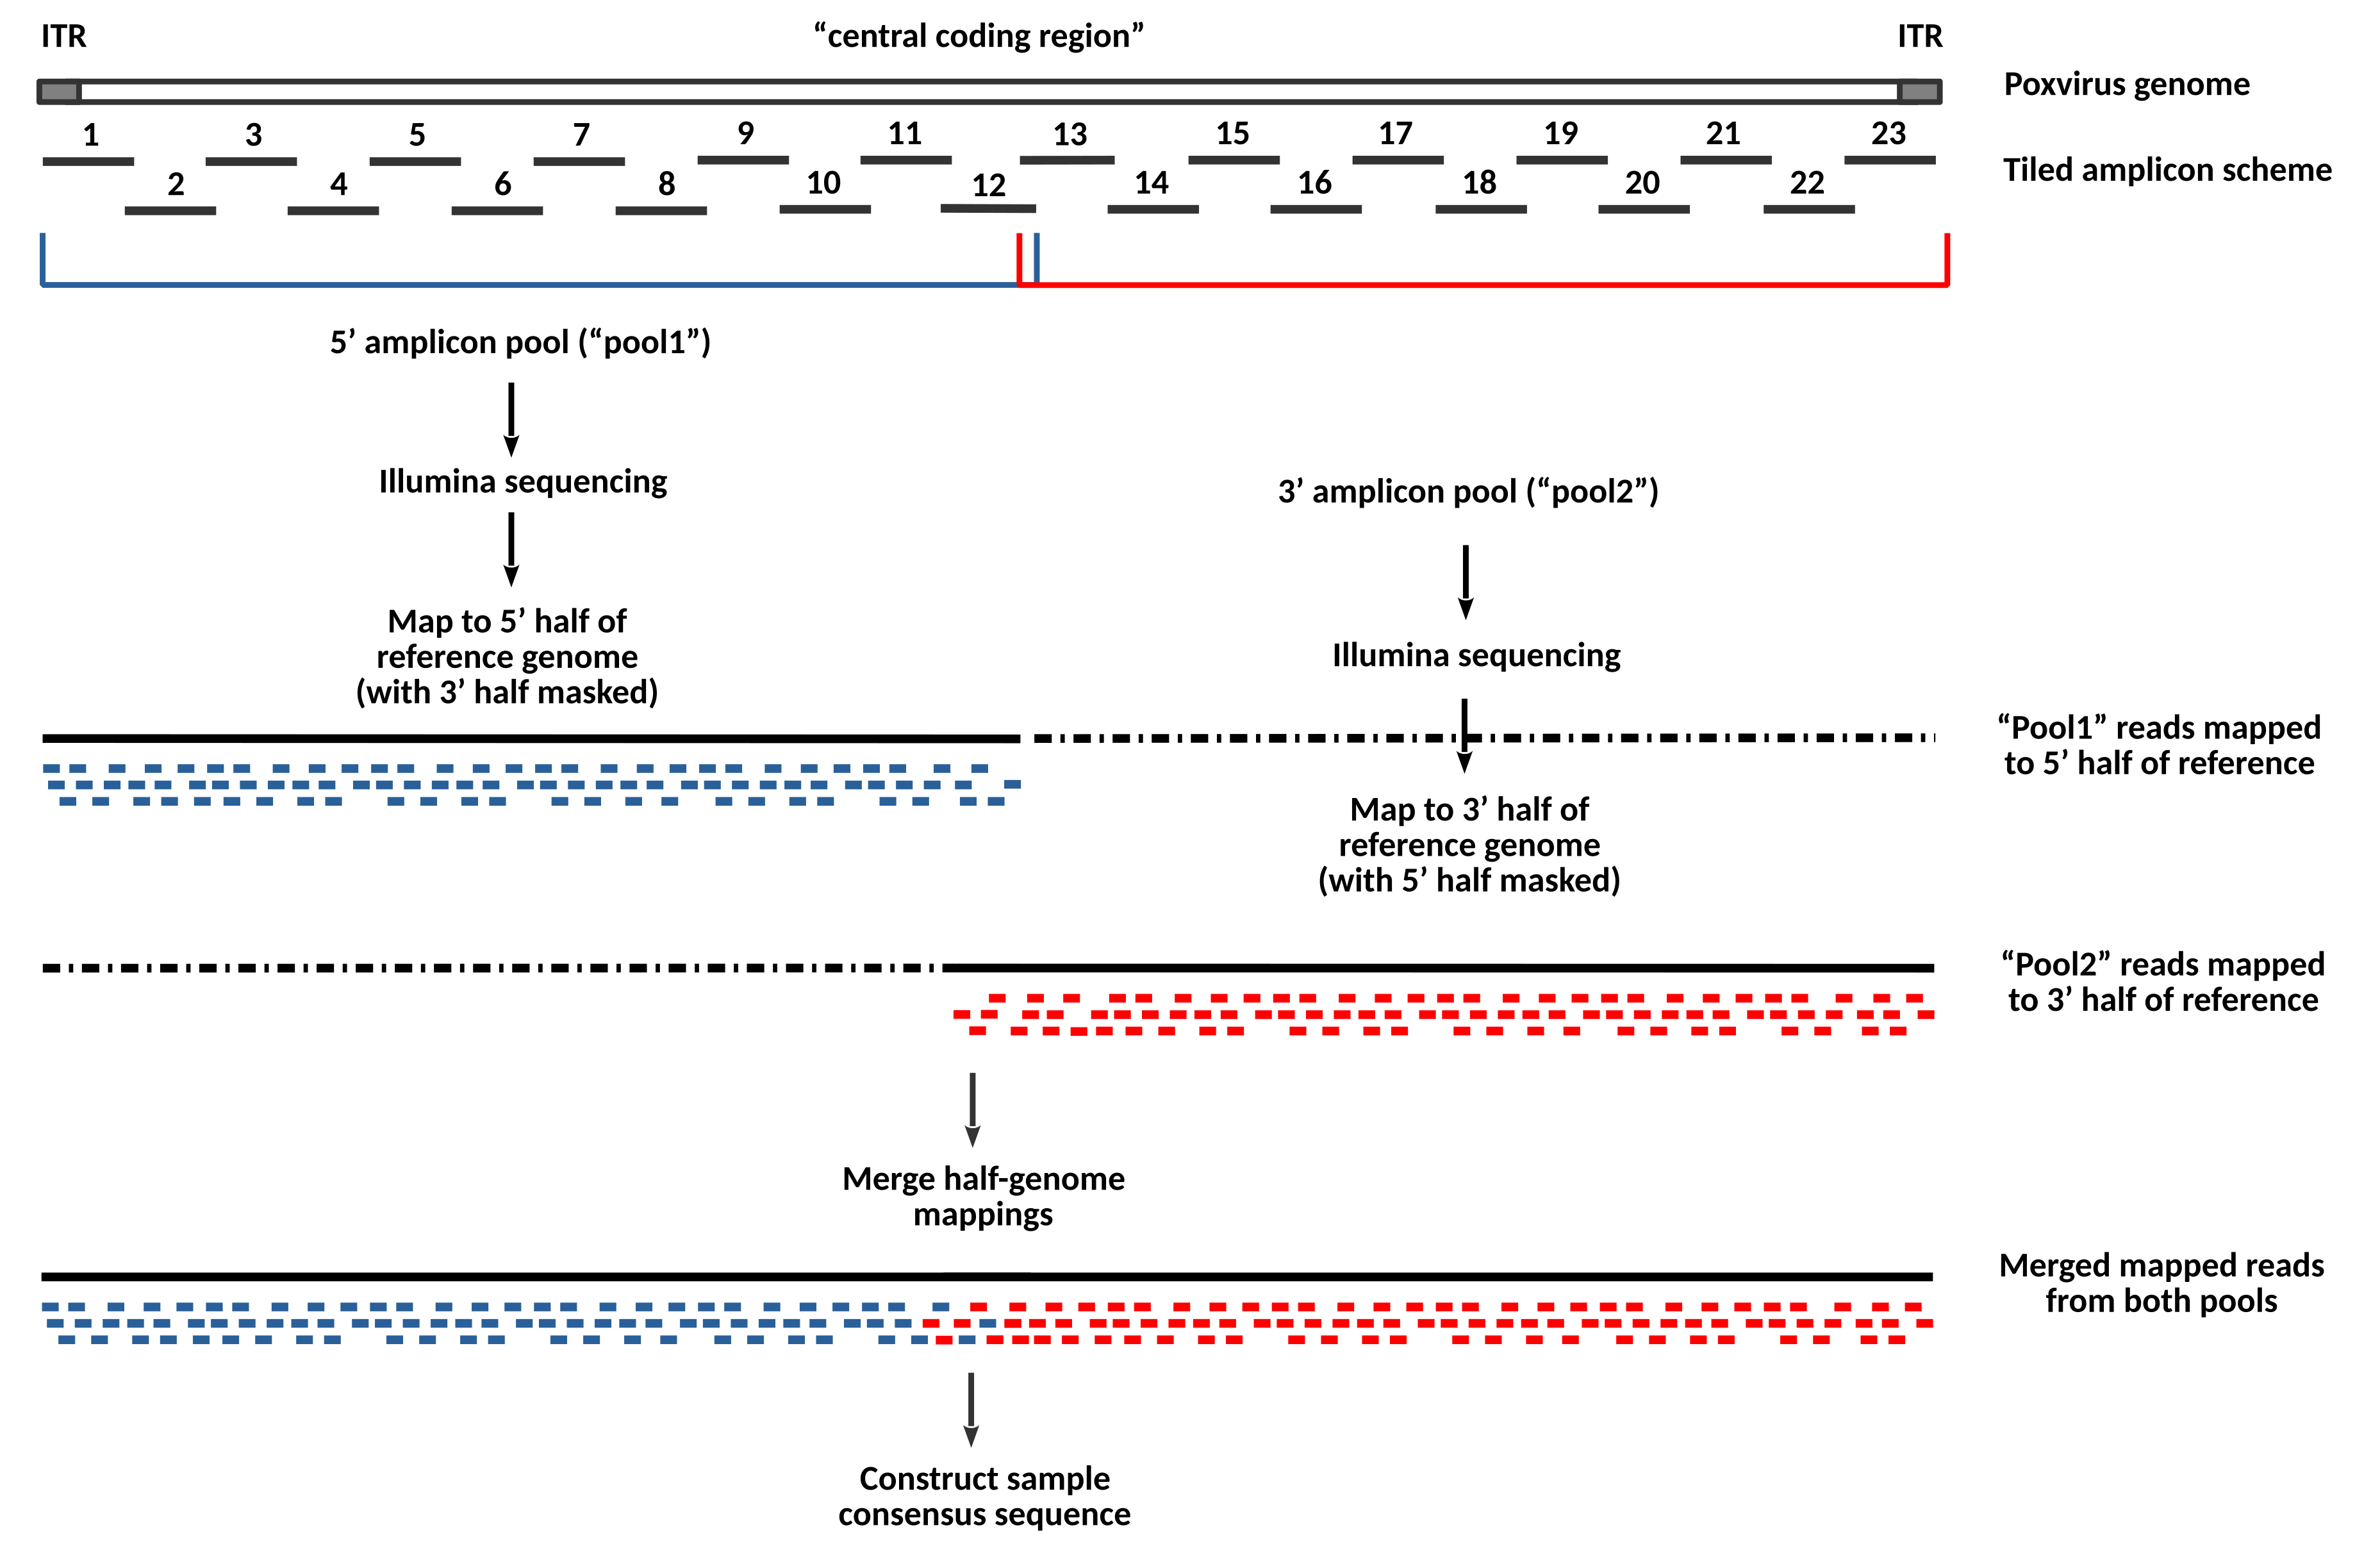
\includegraphics[width=1.1\textwidth]{media/4-pox-ampl-fig.png}
    \caption[Tiling amplicon scheme used in poxvirus workflow.]{Tiling amplicon scheme emphasising masking of the reference, mapping in two pools and merging of mappings with almost no overlap.}
    \label{fig:4-pox-ampl}
\end{figure}
The used primer scheme contains a total of 23 primers, while the first set of 12 primers covers the 5' genome and are labeled with \textit{pool1} and the remaining 11 primers cover the 3' genome half, labeled with \textit{pool2} as depicted in blue (\textit{pool1}) and red (\textit{pool2}) in~\figref{fig:4-pox-ampl}. This scheme was designed for the tiling amplicon approach and allows to generate the complete genome of all three members of Capripoxviruses, which includes the \ac{LSDV} sample. The primer scheme works with all Capripoxviruses due to the serological similarity they have. The primer scheme is provided in the Galaxy history of the test runs and is available via links in Supplementary~\secref{sec:apx-pox-links}. Inspection  of the masking intervals for N-masking the reference confirms that the right-most position of Ns of masking the 5' half (i.e. preparing the reference for mapping \textit{pool2} reads) is the minimal start position of \textit{pool2} primers (``1 -- 79081'', and 79081 being the start position of primer 13). Accordingly for N-masking the reference for mapping of \textit{pool1} reads, the interval from the right-most primer-end of \textit{pool1} primers is 80202, the end position of primer 12, resulting in the interval ``80202 -- 150773''. This is clearly visible in~\figref{fig:4-lsdv-read-groups}, where reads from \textit{pool1} are labeled in red and \textit{pool2} in blue.
The final position is the maximal end position and the total length of the reference sequence. Since the reference genome and primer scheme are the same for both datasets 20L70 and 20L81, the N-masked references are used for both mappings. Mapping of each pool is done with \texttt{BWA-MEM} and default settings for Illumina-sequenced reads, using the N-masked reference for \textit{pool1} and \textit{pool2} respectively. This results in a mapping with a small overlap in the central part of the genome, where primer 12 ends and primer 13 starts as indicated in~\figref{fig:4-pox-ampl}. After merging the mappings with \texttt{Samtools merge}, statistics for preprocessing and mapping are reported and summarised in~\tabref{tab:4-pox-metrics}. For both samples 20L70 and 20L81, almost the complete reference genome was covered during mapping (99.68\%) with a mean coverage of 2705.2 and 2411.4 \texttimes respectively. 
\\

\begin{figure}[ht!]
    \centering
    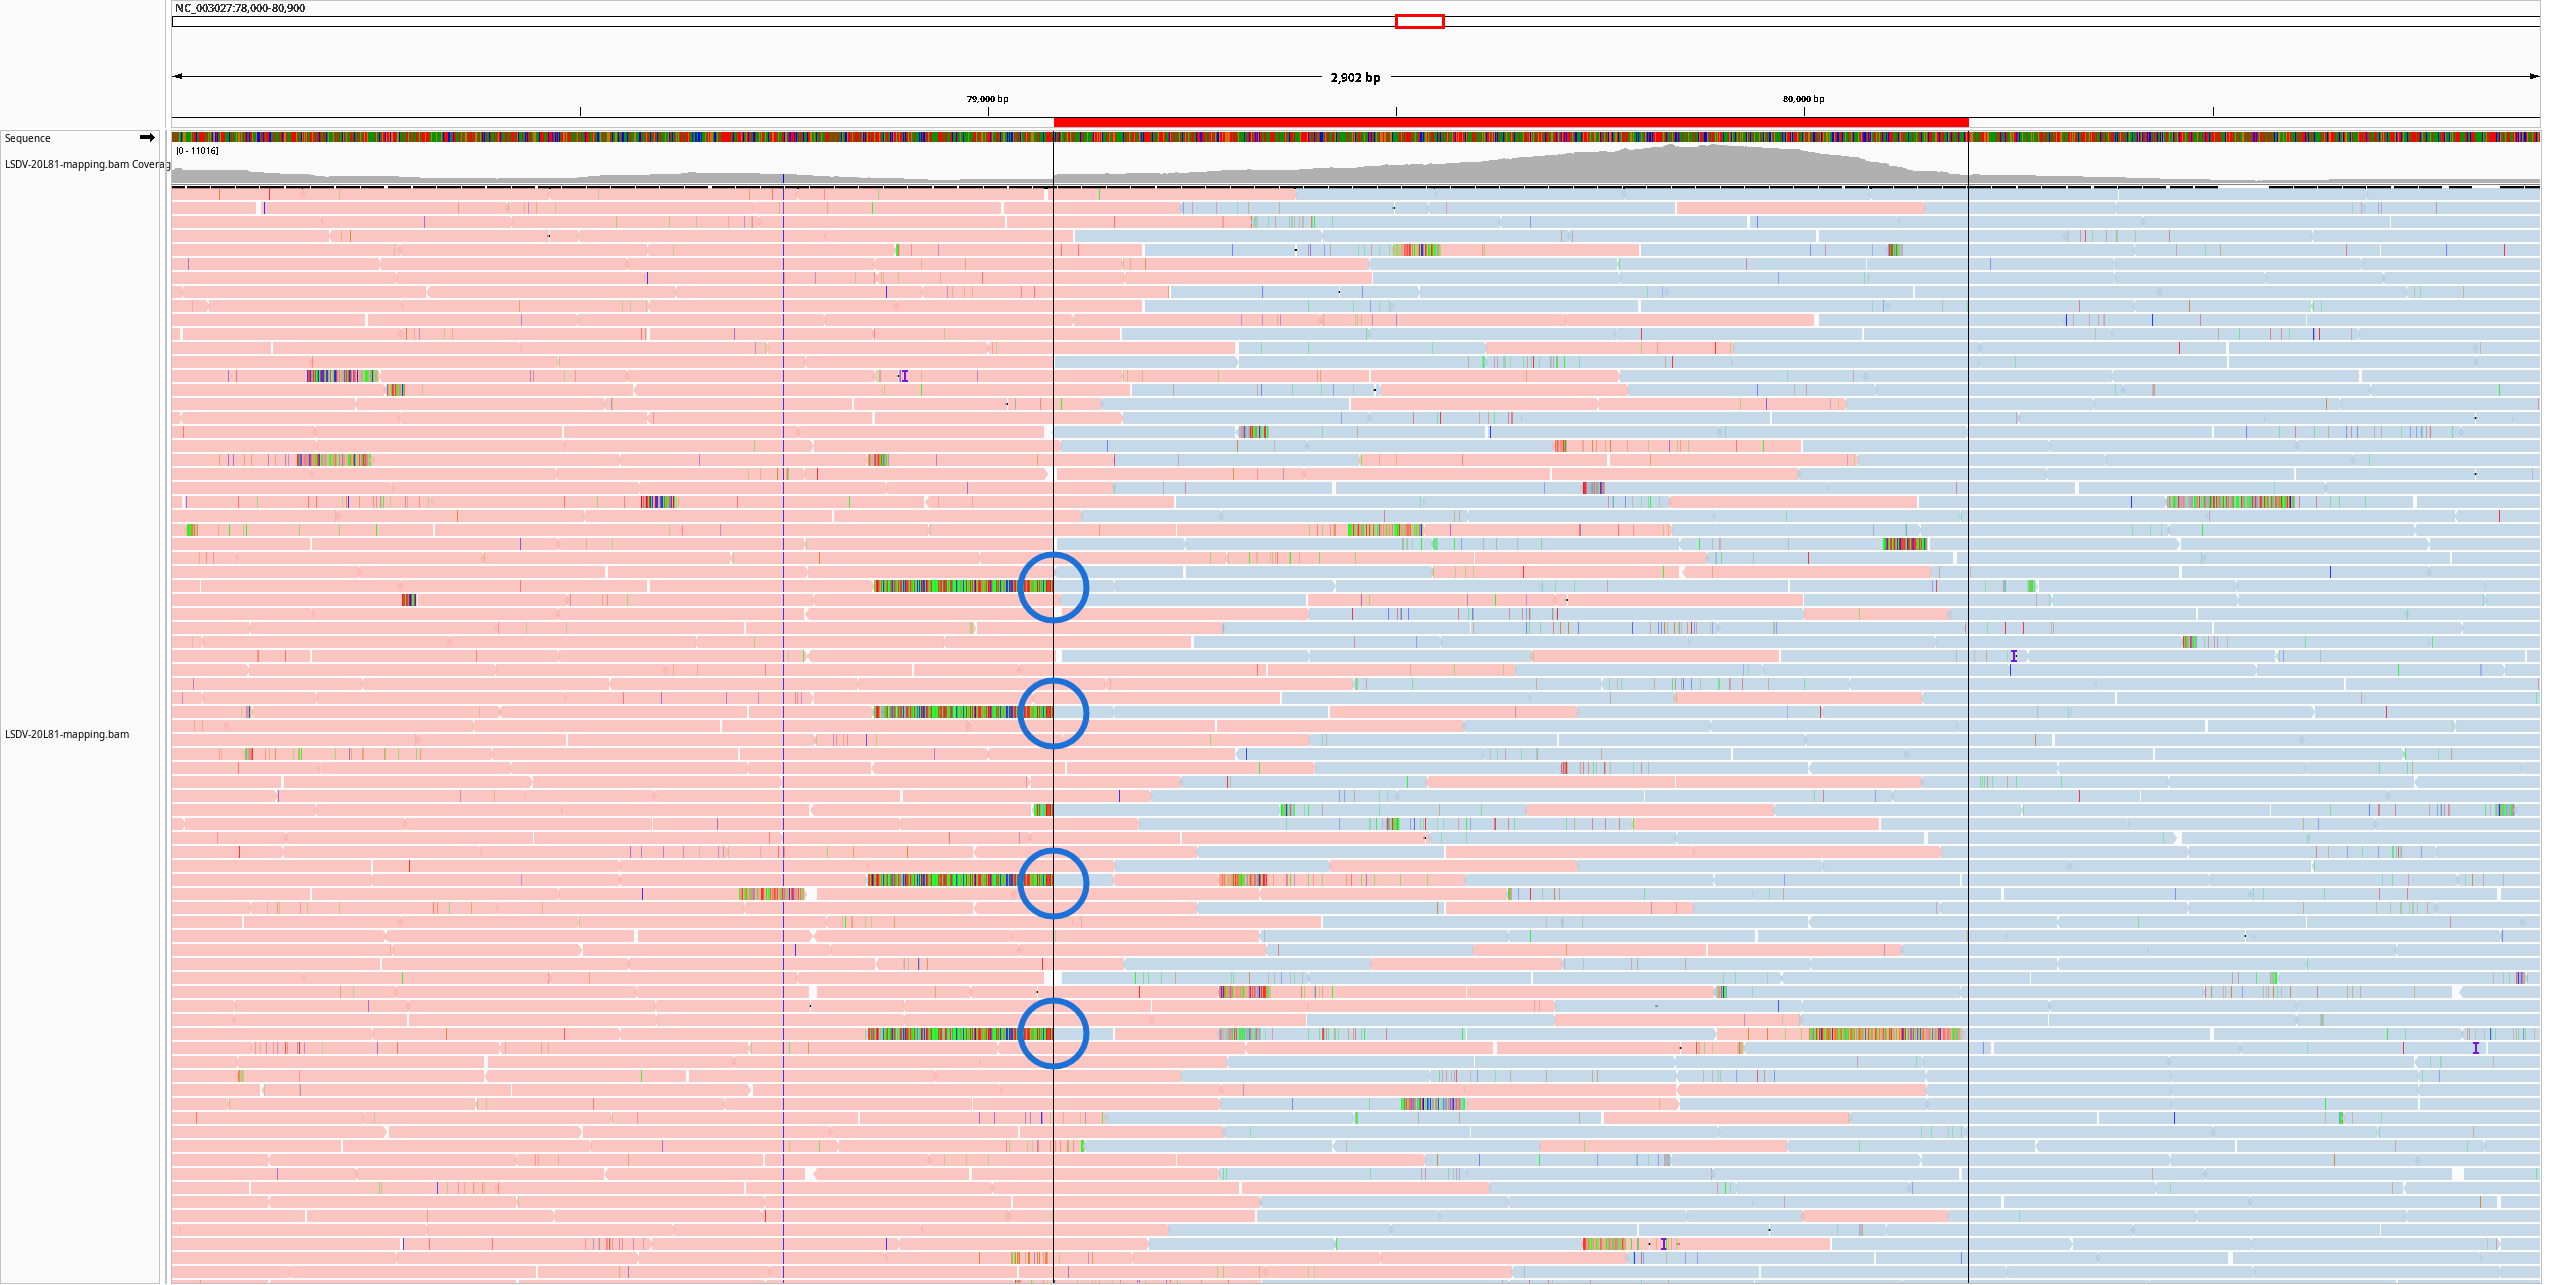
\includegraphics[width=1.0\textwidth]{media/4-lsdv-alig-20L81-c.png}
    \caption[Overlap region of LSDV mapping in 20L81 sample.]{Overlapping, seamlessly merged mapping region of the two amplicon pools of the 20L81 sample. Red and blue reads indicate mapped reads from the respective pool, primers are soft-clipped and end where the mapping of \textit{pool2} reads starts (indicated with blue circles for primer 13 to which four reads from \textit{pool2} bind in this snap).}
    \label{fig:4-lsdv-read-groups}
\end{figure}

The merged mapping of both read pools is quality trimmed with \texttt{iVar trim} to remove primers and reads with a length of less than 30. The remaining reads are used for full-length consensus sequence construction with \textit{iVar consensus}, developed for amplicon-based sequencing data. Inspection of the consensus sequences for both samples shows that apart from low coverage regions in the 5' front and 3' tail due to ampliconic sequencing, a consensus sequence was produced and a base at each position could be found. Ns were called in the consensus at the first 264 positions of each sample which corresponds to the primer binding site on the forward strand, and Ns at the last 268 positions indicate the remaining part where the last primer on the reverse starts because coverage criteria outside of the amplicons was not met in these regions.

% Consensus Sequence
%     20L81
%         front 265 Ns
%         tail 269 Ns
%     20L70
%         front 264 Ns
%         tail 268 Ns

\todo{consensus evaluation: \# of variants with respect to the reference genome (missense variants?)}


\section{AIV Workflow with H4N6 and H5N8 Samples}\label{sec:4-aiv}
\setlength{\tabcolsep}{14pt}
\renewcommand{\arraystretch}{1.3}
\begin{table}[ht!]
    \centering
    \begin{tabular}{lcc} 
    \toprule
    \textbf{Output Metric}                                                                & \textbf{H4N6} & \textbf{H5N8} \\ \midrule
    Paired-end raw reads                                                                  & 1 537 722                  & 858 610                    \\ 
    \begin{tabular}[c]{@{}l@{}}Paired-end reads after quality\\trimming\end{tabular}      & 1 507 396                  & 830 176                    \\ \midrule
    \end{tabular}
    \caption{Metrics after preprocessing of H4N6 and H5N8 samples.}
    \label{tab:4-aiv-metrics}
\end{table}

The \ac{AIV} Illumina workflow on the Galaxy platform was evaluated using two field isolates provided by Sciensano, the Belgian national health institute. The isolates were extracted in Belgium in 2020 from an H4N6 infected magpie (EPI\_ISL\_7593059) and an H5N8 infected duck (EPI\_ISL\_7596571). For reasons of readability, we refer to the samples as H4N6 and H5N8 samples. The two samples were sequenced on an Illumina platform in paired-end mode and are utilised one sample per workflow run on Galaxy. For the \ac{AIV} Illumina workflow, a reference database in FASTA format is required as a collection, i.e. a list of one dataset per \ac{AIV} segment, which is uploaded in Galaxy. The database we used contains multiple sequences per segment as described in~\secref{sec:3-aiv-ref}. The amount of sequences and distribution of subtypes within each segments suggests that variation within each subtype is generally captured well with the given database. Due to the filtering criteria, not all eight segments for one sample were found suitable for the database.\\
After starting the workflow, the paired-end reads are preprocessed and serve as query reads for \texttt{VAPOR}. Metrics are shown in~\tabref{tab:4-aiv-metrics} and count more than 1.50 million reads after preprocessing for the H4N6 sample and 0.83 million reads for the H5N8 dataset. Since the reference database contains eight FASTA files in a collection, \texttt{VAPOR} runs once per dataset and outputs the highest scoring sequences per segment, which represents the most similar sequences from the database to the query sequence. \\

\setlength{\tabcolsep}{8pt}
\renewcommand{\arraystretch}{1.3}
\begin{table}[ht!]
    \centering
    \begin{tabular}{@{}lcccc@{}}
    \toprule
    \multicolumn{1}{c}{\textbf{Segment}} & \multicolumn{2}{c}{\textbf{\% of query bases in reads}}                             & \multicolumn{2}{c}{\textbf{Subtype of hit}}                                         \\ \midrule
                                         & \multicolumn{1}{l}{\textbf{H4N6 sample}} & \multicolumn{1}{l}{\textbf{H5N8 sample}} & \multicolumn{1}{l}{\textbf{H4N6 sample}} & \multicolumn{1}{l}{\textbf{H5N8 sample}} \\ \cmidrule(l){2-5} 
    HA                                   & 98.7                                    & 100.0                                      & H4                                       & H5                                       \\
    NA                                   & 98.7                                    & 100.0                                      & N6                                       & N8                                       \\ \bottomrule
    \end{tabular}
    \caption[Results of the VAPOR run with AIV test samples.]{The best scoring sequence of the VAPOR run for each AIV test samples, indicating a perfect match (100\% of the query bases are in the reads) of the HA and NA segments of the H5N8 sample sequence.}    
\label{tab:4-aiv-vapor}
\end{table}

The \texttt{VAPOR} search was able to successfully identify the avian influenza virus subtypes present in each sample: for the H5N8 sample, the most similar sequence of HA segment origins from a sample with the H5 subtype, while the most similar sequence of the NA segment origins from a sample with the N8 subtype. Both found gene sequences contain 100\% of the input reads. Similarly, the H4N6 sample was correctly identified with concordance of query bases of 98.7\%. The results of the \texttt{VAPOR} run for the HA and NA genes are summarised in~\tabref{tab:4-aiv-vapor}. \\
Consensus sequences for each segment were constructed and while a consensus could be found for each position, they are 100\% identical to the originally assembled reads that were uploaded to \ac{GISAID} from the same sample. Due to slightly different genome sizes of the reference sequence used for mapping compared to the assembly, the resulting consensus sequences in the \ac{AIV} workflow are shorter than the assembled sequences on \ac{GISAID}. The consensus sequence for the \ac{HA} segment of the H4N6 sample is differing in 1 bp in the front 5', and 4 bp in the 3' tail. The consensus sequence constructed for the \ac{NA} gene misses 18 bp compared to the assembled sequence on \ac{GISAID} in the 5' front and 33 bp in the 3' tail. Similarily, the \ac{HA} consensus sequence of sample H5N8 is 28 bp shorter in the front and 44 bp shorter in the end. The \ac{NA} consensus sequence differs in 20 and 28 bp in the front and tail. These differences in length can occur due to different reference sequence length, consensus coverage thresholds or different preprocessing settings. \\
Other workflow outputs for the \ac{AIV} samples include plots that visually emphasise \acp{SNP} relative to the top hits of the \texttt{VAPOR} run, indicating the most similar sequences from the reference collection. The plots for the \ac{HA} and \ac{NA} genes for the H4N6 sample (\figref{fig:apx-aiv-snipit-s4}) show 30 \acp{SNP} compared to the first sequence which was also used as reference for mapping (LC121412.1) and 31 \acp{SNP} compared to the second best result (MK192399.1). Similarly, the \ac{NA} gene consensus sequence has 29 \acp{SNP} compared to the reference sequence (MW19994.1). For the H5N8 sample, the \texttt{VAPOR} run found a sequence with 100\% of the query bases in the reads, and therefore the number of \acp{SNP} is expected to be low. Supplementary~\figref{fig:apx-aiv-snipit-s8} shows there is one \ac{SNP} in the \ac{HA} gene compared to the reference (MZ166252.1) at position 1002 and one \ac{SNP} at position 497 compared to the \ac{NA} reference sequence (MZ166270.1). The \acp{SNP} can indicate point mutations or errors, low coverage or close calls during consensus sequence construction. \\
Phylogenetic classification relative to the 30 most similar sequences in the \ac{AIV} reference database, queried by \texttt{VAPOR}, is done for each segment to reveal temporal and geographical relations of the isolate. Generated phylogenetic trees with \texttt{IQ-Tree} are depicted in Supplementary Figures~\ref{fig:apx-aiv-trees-s4} and~\ref{fig:apx-aiv-trees-s8}. The trees are unrooted and both for \ac{HA} and \ac{NA} genes, they show the nearest clades being from a isolate which is a H4N6 infected duck from France, taken in 2020. This seems valid regarding the examined sample being from a duck in Belgium, also taken in 2020. Users could investigate in more detail by uploading their own reference collection and hereby finding links to other sequenced samples from previous outbreaks in their region. The depth of the split in a phylogenetic tree can indicate the degree of relatedness between the sample and the other samples within that split. A deeper split suggests a closer relationship between the sample and the other samples in that particular branch.

\section{FMDV Workflows with Asia-1, A, SAT-1 and SAT-2 Samples}
The samples used for workflow validation are downloaded from the \ac{NCBI} and were chosen exemplatory for four of the seven different \ac{FMDV} serotypes. All four samples were sequenced on an Illumina NextSeq 550 platform. Two samples (Asia-1 serotype, SRR17960053 and A serotype, SRR18751245) were taken from infected cattle and buffalo during an outbreak in Pakistan from 2008 to 2012. One sample (SAT-1 serotype, SRR18685689) was isolated from buffaloes in Kenya in 2016 and plaque purified before sequencing, and the fourth sample (SAT-2 serotype, SRR9328470) was taken from an \ac{FMD} outbreak in Nigeria in 2014. \\
The metrics for preprocessing of the raw reads are described in~\tabref{tab:4-fmdv-metrics}. The SAT-2 sample contains a very low number of reads with only 11 576 reads after preprocessing, however to show the ability of the developed workflows, it was kept in the test sample collection. 
\\

\setlength{\tabcolsep}{12pt}
\renewcommand{\arraystretch}{1.3}
\begin{table}[ht!]
    \centering
    \begin{tabular}{lcccc} 
    \toprule
    \textbf{Output Metric}                                                              & \textbf{Asia-1} & \textbf{A}                                           & \textbf{SAT-1} & \textbf{SAT-2}\\ \midrule
    Paired-end raw reads                                                                & 577 360         & 2 297 706                                            & 903 052        & 11 816        \\ 
    \begin{tabular}[c]{@{}l@{}}Paired-end reads after quality\\trimming\end{tabular}    & 561 280         & 2 112 856                                            & 806 712        & 11 576        \\ \midrule
    \begin{tabular}[c]{@{}l@{}}Length of assembled contigs\\with > 4000 bp\end{tabular} & 7 760            & \begin{tabular}[c]{@{}l@{}}12 133\\7 558\end{tabular}  & 7 329           & 7 696          \\ \bottomrule
    \end{tabular}
    \caption{Metrics after preprocessing and \textit{de novo} assembly of Asia-1, A, SAT-1 and SAT-2 serotype reads.}
    \label{tab:4-fmdv-metrics}
\end{table}

After \textit{de novo} assembly with \texttt{rnaviralSPAdes}, contigs less than half the length of the \ac{FMDV} genome size were discarded. This resulted in one contig per sample for the \ac{BLAST}n search, except for the A serotype reads, for which two contigs were assembled. As the longer contig with 12 133 bases is far larger than the \ac{FMDV} genome size, a contamination or co-infection with another virus is indicated. The \ac{BLAST}n search was performed against the \ac{NCBI} nucleotide database to identify the closest viral sequence matches. The results of the \ac{BLAST}n search showed that all the contigs were closely related to \ac{FMDV} as listed in~\tabref{tab:4-fmdv-blast}. The highest sequence identity was observed for the Asia-1 serotype sample, with 96.736\% identity, followed by the A, SAT-1 and SAT-2 serotypes, with 94.870\%, 93.766\% and 91.420\% identity, respectively. These results were consistent with the clinical samples being positive for \ac{FMDV} infection and the specific serotype. However, the second contig of the A sample resulted in a \ac{BLAST}n hit for pestivirus (formerly known as bovine viral diarrhea virus 1) with 93.162\% identity~\cite{smith2017proposed}. This suggests the presence of a co-infection with the pestivirus in the sample. It shows that the presented workflow is capable of assembling and identifying other viruses present in a sample. For the consensus sequence construction in the second \ac{FMDV} workflow, the presence of the pestivirus can be ignored and the reference for mapping can be chosen from the \ac{FMDV} hits for the other contig in the \ac{BLAST}n search. However it shows that the user is required to attentively check the results for plausibility and the reference selection process should not be automated without exact validation of the desired virus. Note that \ac{BLAST} runs on the Galaxy EU servers use a locally installed database to ensure replicability of experiments. Hence results on the web form of the \ac{NCBI} \ac{BLAST}n search may result in different hits due to a different database state. In the megablast search made in this workflow, the \ac{NCBI} NT database from 22\textsuperscript{nd} January 2018 was used. The multisample run with the discussed samples of this first \ac{FMDV} workflow is provided in a Galaxy history and is available via link, see Supplementary~\secref{sec:apx-fmdv-links}.

\setlength{\tabcolsep}{12pt}
\renewcommand{\arraystretch}{1.3}
\begin{table}[ht!]
    \centering
    \begin{tabular}{@{}lcccc@{}}
    \toprule
    \textbf{Sample} & \textbf{\begin{tabular}[c]{@{}c@{}}Alignment length\\{[}bases{]}\end{tabular} }   & \textbf{\begin{tabular}[c]{@{}c@{}}Query coverage\\{[}\%{]}\end{tabular} } & \textbf{\begin{tabular}[c]{@{}c@{}}Identical matches\\{[}\%{]}\end{tabular}} \\ \midrule
    A              & 7602   & 92.213  & 94.870      \\
    Asia-1         & 7690   & 99.098  & 96.736      \\
    SAT-1          & 7331   & 100.0   & 93.766      \\
    SAT-2          & 7669   & 99.649  & 91.420      \\ \bottomrule
    \end{tabular}
    \caption[Results of the BLASTn run with four FMDV samples.]{Results of the BLASTn run with four FMDV samples. Query coverage refers to the percentage of identical matches in the alignment compared to the BLASTn hit, hereby indicating the quality of the alignment. Alignment length describes the alignment compared to the query length, indicating how much of the query sequence is covered with the alignment.}
\label{tab:4-fmdv-blast}
\end{table}

In order to run the second workflow for reference-based mapping and consensus sequence construction for each of the four samples, the top \ac{BLAST}n hit of each sample is downloaded in FASTA format to be used as reference sequence for the respective sample. Except for the A sample, the top hit is a \ac{FMDV} genome sequence of the serotype of the query sample. In this case, user control is crucial for the selection of a representative reference sequence of the respective virus and not the contaminating viral sequence.\\
With the \texttt{NCBI Accession Download} tool, the reference sequences are added to the Galaxy history and with \texttt{Collapse Collection} the FASTA file is extracted from the list to a single file, so that it is in the required format for the second \ac{FMDV} workflow.\\

\setlength{\tabcolsep}{8pt}
\renewcommand{\arraystretch}{1.3}
\begin{table}[ht!]
    \centering
    \begin{tabular}{@{}lllll@{}}
    \toprule
    \textbf{Output Metric}                                                            & \textbf{Asia-1}    & \textbf{A}          & \textbf{SAT-1}     & \textbf{SAT-2}   \\ \midrule
    \begin{tabular}[c]{@{}l@{}}Accession no. of\\reference\end{tabular}               & KM268898.1         & JN006722.1          & KM268899.1         & JX014256.1       \\ \midrule
    \begin{tabular}[c]{@{}l@{}}Proportion of reads\\mapping to reference\end{tabular} & 100\%              & 100\%               & 100\%              & 100\%            \\
    \begin{tabular}[c]{@{}l@{}}Proportion of reference\\covered\end{tabular}          & 99.67\%            & 100\%               & 98.16\%            & 99.60\%          \\ \midrule
    Mean coverage                                                                     & 1 525.9 \texttimes & 15 895.5 \texttimes & 9 302.8 \texttimes & 188.0 \texttimes \\
    Alignment error rate                                                              & 3.47\%             & 5.08\%              & 5.87\%             & 8.18\%           \\ \bottomrule
    \end{tabular}
    \caption{Quality and coverage metrics of the alignment in the second FMDV workflow.}
\label{tab:4-fmdv-map}
\end{table}

For each of the testing samples, the accession numbers used as references for mapping with \texttt{BWA-MEM} are listed in~\tabref{tab:4-fmdv-map} as well as quality and coverage measures after mapping. As expected due to the low number of reads, the SAT-2 sample had a low mean coverage of 188.0 \texttimes and a relatively high error rate of 8.18\% compared to the other samples. Consensus sequences are accurately obtained for the Asia-1 and SAT-1 sample that each contain low-coverage regions in the 5' front and 3' tail, so the consensus was lost with decreasing coverage in both genomic ends. Sample A has its only low coverage region immediately adjacent to the polyA tail at positions 7626--7634. The Asia-1 and SAT-1 samples show additional low coverage regions adjacent to the polyC tract (Asia-1 sample: genomic positions 372--383; SAT-1: 321--335). Using the same coverage threshold for consensus calling for a low reads sample like SAT-2, the coverage criteria were not met in several regions (genomic positions 1--37, 293, 346--528, 3605--3639 and 8039--9131). The consensus sequences can be found in the Galaxy histories of the respective workflow runs for each sample which are linked in Supplementary~\secref{sec:apx-fmdv-links}.

% \section{Workflow Profiling}
% \todoit and add to methods
% Assembly vs. mapping? blast, vapor
